\documentclass[ignorenonframetext, professionalfonts, hyperref={pdftex, unicode}]{beamer}

\usetheme{Copenhagen}
\usecolortheme{wolverine}

%Packages to be included
%\usepackage{graphicx}

\usepackage[russian]{babel}
\usepackage[utf8]{inputenc}
\usepackage[T1]{fontenc}

%%\usepackage[orientation=landscape, size=custom, width=16, height=9.75, scale=0.5]{beamerposter}

\usepackage{textcomp}

\usepackage{beamerthemesplit}

\usepackage{ulem}

\usepackage{verbatim}

\usepackage{ucs}


\usepackage{listings}
\lstloadlanguages{bash}

\lstset{escapechar=`,
	extendedchars=false,
	language=sh,
	frame=single,
	tabsize=2, 
	columns=fullflexible, 
%	basicstyle=\scriptsize,
	keywordstyle=\color{blue}, 
	commentstyle=\itshape\color{brown},
%	identifierstyle=\ttfamily, 
	stringstyle=\mdseries\color{green}, 
	showstringspaces=false, 
	numbers=left, 
	numberstyle=\tiny, 
	breaklines=true, 
	inputencoding=utf8,
	keepspaces=true,
	morekeywords={u\_short, u\_char, u\_long, in\_addr}
	}

\definecolor{darkgreen}{cmyk}{0.7, 0, 1, 0.5}

\lstdefinelanguage{diff}
{
    morekeywords={+, -},
    sensitive=false,
    morecomment=[l]{//},
    morecomment=[s]{/*}{*/},
    morecomment=[l][\color{darkgreen}]{+},
    morecomment=[l][\color{red}]{-},
    morestring=[b]",
}

\author[Epam]{{\bf Epam}\\Low Level Programming Department}

%\institution[EPAM]{EPAM}
%\logo{\includegraphics[width=1cm]{logo.png}}


\title{Введение в GNU/Linux}


%%%%%%%%%%%%%%%%%%%%%%%%%%%%%%%%%%%%%%%%%%%%%%%%%
%%%%%%%%%% Begin Document  %%%%%%%%%%%%%%%%%%%%%%
%%%%%%%%%%%%%%%%%%%%%%%%%%%%%%%%%%%%%%%%%%%%%%%%%




\begin{document}

\begin{frame}
	\frametitle{}
	\titlepage
	\vspace{-0.5cm}
	\begin{center}
	%\frontpagelogo
	\end{center}
\end{frame}


%%%%%%%%%%%%%%%%%%%%%%%%%%%%%%%%%%%%%%%%%   
%%%%%%%%%% Content starts here %%%%%%%%%%
%%%%%%%%%%%%%%%%%%%%%%%%%%%%%%%%%%%%%%%%%

\section{Основы работы с сетевой подсистемой}

\mode<all>{\begin{frame}{Сетевая подсистема Linux}

	\begin{block}{Cетевой интерфейс}

		Сетевой интерфейс в Linux -– это абстрактный именованный объект,  используемый для передачи 
		данных через некоторую линию связи без привязки к ее (линии связи) реализации.
	\end{block}
\end{frame}

\begin{frame}{Сетевая подсистема Linux}

	\center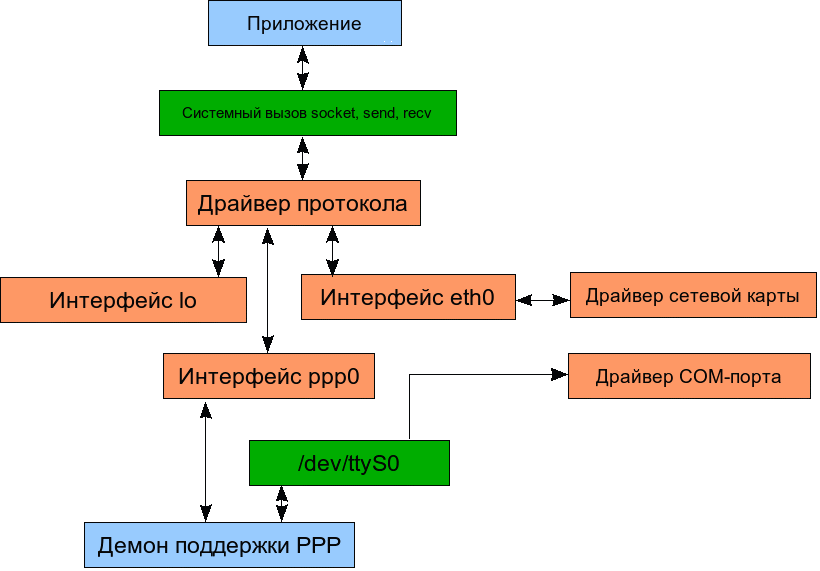
\includegraphics[height=0.8\textheight]{../../slides/networking/06-netstack.png}

\end{frame}


}

\subsection{Управление интерфейсами}
\mode<all>{\begin{frame}{Команды управления настройками сети}
	\begin{itemize}
	  \item ifconfig/route
	  \item iproute2
	\end{itemize}

	\begin{itemize}
		\item Список интерфейсов
			\begin{itemize}
				\item {\tt ifconfig -a}
				\item {\tt ip link show}
			\end{itemize}
		\item Включение интерфейса 
			\begin{itemize}
				\item {\tt ifconfig <iface> up}
				\item {\tt ip link set <iface> up}
			\end{itemize}
	  \item Выключение интерфейса
			\begin{itemize}
				\item {\tt ifconfig <iface> down}
				\item {\tt ip link set <iface> down}
			\end{itemize}
	  \item Назначение адреса
			\begin{itemize}
				\item {\tt ifconfig eth0 192.168.1.17 netmask 255.255.254.0 up}
				\item {\tt ip addr add 192.168.1.17/23 dev eth0}
			\end{itemize}
	\end{itemize}
\end{frame}

\begin{frame}{Конфигурационные файлы}
  \begin{itemize}
    \item {\tt /etc/resolv.conf}
    \item {\tt /etc/hosts}
	\item {\tt /etc/sysconfig/network}
    \item Расположение зависит от дистрибутива:
		\begin{itemize}
			\item RH-like: {\tt /etc/sysconfig/network-scripts}\\
				{\tt /etc/sysconfig/network-scripts/ifcfg-eth0}
			\item ALTLinux: {\tt /etc/net/ifaces}
			\item Debian: {\tt /etc/network/interfaces}
			\item Gentoo: {\tt /etc/conf.d/net}
		\end{itemize}
  \end{itemize}
\end{frame}

\begin{frame}{Дополнительные интерфейсы}
	\begin{block}{Алиасы}
		\begin{itemize}
			\item ifconfig <iface>:<alias> <ip> up
			\item ifconfig <iface> add <ip> up
			\item ip addr add <ip> {\bf label} <iface>:<alias> dev <iface>
		\end{itemize}
	\end{block}
	\pause
	\begin{block}{VLAN}
		\begin{itemize}
			\item vconfig add <iface> <id>
			\item vconfig rem <iface>{\bf.}<id>
			\item ip link add {\bf link} <iface> name <vlan\_name> {\bf type vlan id <id>}
			\item ip link delete <vlan\_name>
		\end{itemize}
	\end{block}

\end{frame}


}

\subsection{Полезные программы}
\mode<all>{\begin{frame}{Полезные утилиты}
	\begin{center}
		\begin{itemize}
			\item netstat / ss
			\item nslookup / dig
			\item ping
			\item traceroute
			\item tcpdump
			\item telnet
			\item netcat
			\item nmap
		\end{itemize}
	\end{center}

\end{frame}


\begin{frame}[allowframebreaks]{Полезные утилиты: практика}

		\begin{block}{netstat}

			Узнать:
			\begin{itemize}
				\item список используемых сокетов
				\item серверных сокетов
				\item имена/pid серверов
				\item узнать номера портов
			\end{itemize}
		\end{block}
	
		\framebreak
		\begin{block}{telnet/netcat}

			\begin{itemize}
				\item Чат по протоколу TCP с соседом
				\item Чат по протоколу UDP с соседом
				\item Передать текстовый и бинарный файлы
			\end{itemize}
	
			При создании чата использовать {\tt netstat} и {\tt tcpdump}
			для получения информации о соединении.
		\end{block}

		\framebreak
		\begin{block}{nmap}
			\begin{itemize}
				\item сканирование соседа
				\item сканирование выделенных портов у соседа (поиск сервера чата) 
				\item узнать список открытых портов на всех машинах в аудитории
				\item узнать список работающих машин
			\end{itemize}
		\end{block}
	
\end{frame}

tcpdump
0. pcap файлы/libpcap
1. запуск монитора
2. запуск чата
3. монитор-фильтр-анализ

}

\section{ssh}
\mode<all>{\begin{frame}{ssh}

	\begin{block}{ssh -- терминал}
		{\tt ssh [user@]host[:port]}\\
		{\tt ssh host [-l user] [-p port]}
		\begin{itemize}
			\item -v -- "разговорчивый" режим 
			\item -t -- насильное назначение псевдотерминала (для автоматизации)
		\end{itemize}
		Вся конфигурация пользователя: {\tt \$HOME/.ssh}
	\end{block}

	\pause

	\begin{block}{... и не только}
		\begin{itemize}
			\item -X -- "проброс" графики 
			\item -L [bindip:]port:rhost:rport -- "пробрасывание" порта с удаленной машины на локальную
			\item -R [bindip:]port:lhost:lport -- "пробрасывание" порта с локальной машины на удаленную
			\item -W host:port -- stdin/stdout с указанным хостом
			\item -D port -- динамический прокси
		\end{itemize}
	\end{block}
\end{frame}


}


\section{Дополнительные типы интерфейсов}

\subsection{alias, vlan}
\mode<all>{
\begin{frame}{Дополнительные интерфейсы}
	\begin{block}{Алиасы}
		\begin{itemize}
			\item ifconfig <iface>:<alias> <ip> up
			\item ifconfig <iface> add <ip> up
			\item ip addr add <ip> {\bf label} <iface>:<alias> dev <iface>
		\end{itemize}
	\end{block}
	\pause
	\begin{block}{VLAN}
		\begin{itemize}
			\item vconfig add <iface> <id>
			\item vconfig rem <iface>{\bf.}<id>
			\item ip link add {\bf link} <iface> name <vlan\_name> {\bf type vlan id <id>}
			\item ip link delete <vlan\_name>
		\end{itemize}
	\end{block}

\end{frame}


}
\subsection{Мосты}
\mode<all>{\begin{frame}{Мосты}
	\begin{itemize}
		\item Создать -- {\tt brctl addbr <bridge>}
		\item Удалить -- {\tt brctl delbr <bridge>}
		\item Добавить интерфейс -- {\tt brctl addif <bridge> <device>}
		\item Удалить интерфейс-- {\tt brctl addif <bridge> <device>}
	\end{itemize}
\end{frame}


}
\subsection{Виртуальные}
\mode<all>{
\begin{frame}{''Виртуальные'' интерфейсы}
	\begin{block}{TUN/TAP}

		{\tt modprobe tun}

		\begin{itemize}
			\item Добавить интерфейс TUN -- {\tt tunctl -n -t <ifacename>}
			\item Добавить интерфейс TAP -- {\tt tunctl -p -t <ifacename>}
			\item Удалить интерфейс -- {\tt tunctl -d <ifacename>}
		\end{itemize}
	\end{block}

	\pause

	\begin{block}{Практика}
		\begin{itemize}
			\item Создать интерфейс TAP с именем {\tt mytap}
			\item Создать мост с именем {\tt mybr}
			\item Назначить интерфейсу {\tt mytap} адрес {\tt 192.168.0.<n>/24}
			\item Добавить интерфейсы {\tt mytap} и {\tt eth0} к мосту {\tt mybr}
			\item Запустить {\tt tcpdump} на интерфейсах {\tt mybr} и {\tt mytap}
			\item Запустить {\tt ping} соседа
		\end{itemize}
	\end{block}

\end{frame}


}
\mode<all>{\begin{frame}{''Псевдо-ethernet'' интерфейсы}
	\begin{block}{macvlan}
        Виртуальный ethernet интерфейс.\\
        Фактически работает, как копия физического интерфейса со своим MAC-адресом.
	\end{block}

	\begin{block}{iproute2}
		\begin{itemize}
			\item Добавить интерфейс macvlan -- \\
                {\tt ip link add name <ifacename> link <parent> type macvlan}
			\item Удалить интерфейс -- \\ 
                {\tt ip link del <ifacename>}
		\end{itemize}
	\end{block}

\end{frame}

}
\mode<all>{\begin{frame}{''Виртуальные пары''}
	\begin{block}{veth}
        Соединение вида точка-точка, с двумя виртуальными ethernet-интерфейсами.
	\end{block}

	\begin{block}{iproute2}
		\begin{itemize}
			\item Создать пару интерфейсов -- \\
                {\tt ip link add name <ifacename1> type veth peer name <ifacename2>}
			\item Удалить (достаточно удалить любой интерфейс) -- \\
                {\tt ip link del <ifacename> }
		\end{itemize}
	\end{block}

\end{frame}

}

\mode<all>\begin{frame}[fragile]{Вопросы?}
    \setcounter{tocdepth}{2}
    \tableofcontents

    \bigskip

    \hrulefill
    \begin{columns}
    \column{0.7\textwidth}
            \center{Материалы:}
            \url{https://yadi.sk/d/Ixp8kHfl3MipCq}
    \column{0.2\textwidth}
        \begin{center}
            
\includegraphics[width=0.7\textwidth]{url-qr-2017}
        \end{center}
    \end{columns}

    Исходники: \url{https://github.com/epam-llpd/linux_courses}

\end{frame}

\end{document}
